\documentclass[english]{textolivre}

% metadata
\journalname{Texto Livre}
\thevolume{17}
%\thenumber{1} % old template
\theyear{2024}
\receiveddate{\DTMdisplaydate{2023}{8}{30}{-1}}
\accepteddate{\DTMdisplaydate{2024}{4}{8}{-1}}
\publisheddate{\DTMdisplaydate{2024}{5}{3}{-1}}
\corrauthor{Luciana Cabrini Simões Calvo}
\articledoi{10.1590/1983-3652.2024.47921}
%\articleid{NNNN} % if the article ID is not the last 5 numbers of its DOI, provide it using \articleid{} commmand 
% list of available sesscions in the journal: articles, dossier, reports, essays, reviews, interviews, editorial
\articlesessionname{dossier}
\runningauthor{Calvo and Hartle}
%\editorname{Leonardo Araújo} % old template
\sectioneditorname{Daniervelin Pereira}
\layouteditorname{João Mesquita}

\title{Virtual exchange in teacher education programs from Brazil and USA: outcomes and challenges}
\othertitle{Intercâmbio virtual em programas de formação de professores do Brasil e EUA: resultados e desafios}

\author[1]{Luciana Cabrini Simões Calvo~\orcid{0000-0001-8145-0588}\thanks{Email: \href{mailto:lcsimoes@uem.br}{lcsimoes@uem.br}}}
\author[2]{Lynn C. Hartle~\orcid{0000-0002-9268-3309}\thanks{Email: \href{mailto:lch1@psu.edu}{lch1@psu.edu}}}
\affil[1]{Universidade Estadual de Maringá, Maringá, PR, Brasil.}
\affil[2]{The Pennsylvania State University, Brandywine, United States of America.}

\addbibresource{article.bib}

\begin{document}
\maketitle
\begin{polyabstract}
\begin{abstract}
Virtual exchanges (VE) are important initiatives to
include pre-service teachers (PST) in internationalization practices
with others at a geographic distance while they remain in their own
contexts of learning (Internationalization at Home -- \cite{beelen2015redefining}. VEs contribute to the development of intercultural and global attitudes as well as foster digital and technological competencies. This paper shares the results of a 2022 and 2023 VE eight-week project with pre-service teachers enrolled in second language acquisition-related courses at state universities, one in the US and one in Brazil. This
article analyzed data from periodic and end-of-semester surveys and
narratives as well as from their interactions and tasks in different
digital platforms to explore the outcomes and challenges of the VE. The
results discuss the perspective of the involved professors and students
as well as established VE teacher education contexts (such as \textcite{hanks2019research,godwin-jones2019telecollaboration} to share insights regarding the virtual exchange experience on PST's global perspective-taking about teacher education and language teaching. Qualitative analysis revealed patterns of desired student outcomes: interactional skills; the development of information, communication technology skills; intercultural
communicative competence; content, cultural, language learning, and
contextual knowledge. Analyses also illustrated the challenges to those
outcomes, such as busy schedules, class format, and difficulties in
communications and interactions.

\keywords{Brazil and US \sep Virtual exchange (VE) \sep Pre-service
	teachers (PST) \sep Second language acquisition (SLA) \sep Outcomes and
	challenges}
\end{abstract}

\begin{portuguese}
\begin{abstract}
Intercâmbios virtuais (IV) são iniciativas importantes
para incluir professores em formação inicial em práticas de
internacionalização com outras pessoas em distâncias geográficas
enquanto permanecem em seus próprios contextos de aprendizagem
(Internacionalização em Casa -- \cite{beelen2015redefining}. IVs contribuem
para o desenvolvimento de atitudes interculturais e globais assim como
promovem competências digitais e tecnológicas. Este artigo compartilha a
experiência de um projeto de oito semanas de IV, realizado em 2022 e
2023, com professores em formação inicial matriculados em disciplinas
relacionadas à aquisição de segunda língua, nos EUA e no Brasil. Dados
de questionários e narrativas assim como das suas interações e tarefas
em diferentes plataformas digitais são analisados. Os resultados são
discutidos considerando a perspectiva dos professores e estudantes
envolvidos assim como de outros estudos de IV (\emph{e.g}. \textcite{hanks2019research,godwin-jones2019telecollaboration} para compartilhar as percepções relacionadas à experiência dos professores em pré-serviço e suas visões globais sobre formação docente e ensino de línguas. Os resultados identificados foram relacionados a: habilidades interacionais, desenvolvimentos no âmbito da tecnologia de informação e comunicação e da competência intercultural; conhecimento contextual e do conteúdo; aspectos linguísticos. Os desafios mencionados foram: agendas ocupadas; formato das aulas e dificuldades em comunicação e interação.


\keywords{Brasil e EUA \sep Intercâmbio Virtual \sep Professores
	em formação inicial \sep Aquisição de segunda língua \sep Resultados e desafios}
 
\end{abstract}
\end{portuguese}
\end{polyabstract}

\section{Introduction}\label{sec-intro}

Previous studies by Institutions of Higher Education (IHE) found ongoing
participation in online academic events, webinars, and Virtual Exchange
(VE) continued beyond the COVID-19 pandemic \cite{bowen2021virtual,garces2020upscaling,woicolesco2022internationalization}. Virtual
Exchange (VE) includes the engagement of groups of learners in extended
periods of online intercultural interaction and collaboration with
international peers as an integrated part of their educational programs
and under the guidance of educators and/or facilitators \cite[p.~1]{garces2020upscaling}. For students unable to physically travel for financial or
personal reasons, participation in virtual exchanges serves to
complement physical travel through cross-cultural \enquote{internationalization
at home} (IaH) and provide opportunities to develop intercultural
communicative competence and skills \cite{beelen2015redefining}.

One of these VE approaches is the Collaborative Online International
Learning (COIL) which brings together classes with a shared syllabus and
projects in which participants from universities in different parts of
the world come to collaborate, usually for four to eight weeks and
embedded as part of the classwork. Participants have opportunities to
discuss course materials, solve a problem, compare cultural norms, and
often create a gradable project. Participants can interact synchronously
(in real time) or asynchronous (not in real time) and can engage with
email, in a learning management platform (i.e., Google Classroom),
voice, social media, Padlet, or any other form of Information and
Communications Technology abbreviated as ICT \cite{odowd2018telecollaboration}.

This paper focuses on a VE/COIL project developed by the researchers in
2022 and 2023. The Brazilian professor, when looking for others
interested in projects based on the COIL model, found the corresponding
at a university in the US. The professors saw each
other’s interests and the VE director at the US
university arranged an E-meeting to discuss potential cross-cultural
collaborations. After a series of exchanges and realized common goals,
professors utilized their knowledge of VE task design \cite{kurek2017task} and this VE project was developed and implemented.

This exploratory Scholarship of Teaching and Learning (SoTL) qualitative
research project \cite{stake2005qualitative} studied the VE of students preparing to
be teachers (called Preservice Teachers, abbreviated at PST) who were
enrolled in Second Language Acquisition (SLA) related courses, one in
the US and another in Brazil. In the two years of the VE Project, there
were 77 students participating in the initiative. PST in the US were
studying how to teach children in their classes who had immigrated to
the US and whose first language was not English. PST in Brazil were
studying to be English teachers.

In both years (2022 and 2023), professors planned an eight-week VE
Project embedded into our existing courses considering: the timeline for
the exchanges, the platforms to be used, the tasks to be developed,
introductory activities, the topics for the students'
cross-cultural projects, the forms of assessment, and the rubric. In
2022 with a class in the US and a class in Brazil and then again with
the research design revised in 2023 with two other classes of students
in respective courses, professors organized collaborative teams of PST
(in each team, PSTs from Brazil and US working together).

The aims of the joint research project\footnote{The research project was
	approved by the Ethics Committee of both universities.} carried out by
the authors of this paper were a) to develop and study a collaborative
inquiry project between students and professors from US and Brazil; b)
to study participants' virtual exchange experience and knowledge on
teacher education; language teaching and learning in both countries; c)
to analyze the development of the participants' intercultural
communicative competence (ICC) and learning and d) the investigation of
the different resources they used when communicating with each other and
the benefits and challenges of information and communication
technologies (ICT) for the VE experience.

In this text, we focus on the outcomes and challenges of the VE,
analyzing data from periodic and end-of-semester surveys and narratives
as well as from the PST interactions and tasks in different digital
platforms.
\section{Literature Review}\label{sec-literaturereview}

According to \textcite{odowd2018telecollaboration}, educators involved in VE
initiatives offer their students the opportunity to develop skills such
as intercultural competence and critical thinking while working on
shared subject content through different cultural perspectives. In
teacher education programs, VE projects have been developed with the
following purposes: \enquote{to help the [Pre-service teachers (PST)]
develop digital, linguistic, and communicative skills; to work on
students' reflectivity and propensity for critical thinking, increased
openness, and social inclusion; and to prepare prospective language
teachers for facilitating their own VEs} \cite{grau2019experiential}.
International collaborative practices in teacher education programs have
the potential to develop global and intercultural attitudes in
pre-service teachers to prepare them to experience different
interactions and opportunities in their professional lives \cite{kopish2020leveraging}.
	
\textcite{sadler2016twelve} highlight that the experiences in VE in language
teacher education programs had an impact both on instructors and
pre-service teachers; it changed their mindset and understandings about
telecollaboration as well as their roles in terms of
instructor-pre-service teacher responsibilities in a way that they could
witness a learner-centered pedagogy. Additionally, the authors state
that the use of telecollaboration and the cooperation between the
teachers are also noticed by the students.
	
\textcite{hauck2019virtual} found that when tackling the communication, cultural,
linguistic and/or technical challenges pre-service teachers faced during
VE, they acquired new competencies in terms of behavioral flexibility,
interaction management, messaging skills, and language competence some
of which interrelate with digital competencies.
	
Incentives or opportunities, such as VE, can bring to light the
importance of the ability to communicate effectively and appropriately
in various cultural contexts in an increasingly global society
\cite{deardorff2020manual}. Some of the key components to developing
Intercultural Communication Competence (ICC) include motivation, self-
and other knowledge, mindfulness, cognitive flexibility, and tolerance
for uncertainty \cite{wilberschied_intercultural_2015}. Direct and thoughtful encounters with people, places, and foreign languages such as through VE with students at other colleges are effective ways to begin to develop ICC \cite{idris2019intercultural,lopez2017developing}.
	
Simply engaging PSTs in VE does not guarantee successful intercultural
outcomes. The types of activities, adequate time, and mentoring by the
instructors are critical to the value of virtual experiences and teacher
exchanges \cite{fuchs2022value}; for them to clearly understand
the content their peers from another culture share as well as be able to
critically, and with respect examine the content to discover
similarities and differences between that culture and their own \cite{roarty2021analysis}.
	
Generally, the first task in those projects is to exchange information
about each other to establish trust in the partnership. Then,
collaborative tasks are developed for analysis and comparison. In the
third phase, when it is included, the partners develop \enquote{some kind of
shareable product or artifact} \cite{godwin-jones2019telecollaboration}. A systematic and
well-planned framework with a constructivist lens that affords choices,
both synchronous and asynchronous platforms and tools but also guidance
with ICT can support the ease of cross-cultural collaboration, reduce
frustration, and facilitate student exploration of ideas \cite{calvo2023investigating,hauck2020approaches,kopish2020leveraging}.
		
\textcite{evaluate2019evaluating} found that students problem-solved when
certain tech problems occurred with synchronous tools and then switched
to a texting online social network -- WhatsApp to continue their
communications. When facing obstacles, pre-service teachers challenged
themselves and others to develop these new ICT collaboration skills. To
support their growth, another aspect of the project design should be a
built-in system for ongoing reflection so the PSTs can see the value of
skills and content learned and how they can apply their learning.

\section{Methods}\label{sec-methods}
\subsection{Overview and Demographics}\label{sub-sec-overviewanddemographics}

This exploratory Scholarship of Teaching and Learning (SoTL) joint
research project studied the cross-cultural \enquote{internationalization at
home} through a eight-week (March-May, 2022) Virtual Exchange (VE) of
students preparing to be teachers, pre-service teachers (PST) enrolled in
Second Language Acquisition (SLA) related courses in the state of
Pennsylvania in the US (18 PST) and in the Paraná state, Brazil (16
PST). The VE initiative was carried out with another group of PST
(March-April, 2023; US= 21 PST; Brazil =22 PST) with
some adjustments based on findings in 2002.

The US course is focused on English as a Second Language (ESOL). The
state certification in Pennsylvania requires that PSTs in all teaching
disciplines take courses (at least 90 hours of study) to prepare for
teaching children who immigrate to the US with minimal English skills
since these children spend 90\% of their day in non-bilingual
classrooms. The course is taken in their second or third year of their
studies. Most US PSTs were not bilingual (N=35\% bilingual) and for
those who were bilingual, predominantly the first language was Spanish
and none spoke Portuguese. The course format was asynchronous web-based
enrolling PSTs from several regions of the state.

In Brazil, the group of students were enrolled in the course \enquote{English
Teacher Education Practice} in the third year of their undergraduate
curriculum. They are from the Language Arts undergraduate Program
(English major) and they were studying to be English teachers (See \Cref{tab-01}).
		
		

\begin{table}[htpb]
\centering
\begin{threeparttable}
\caption{Courses in US and Brazil and their respective enrollments.}
\label{tab-01}
\small
\setlength{\tabcolsep}{3pt}
\begin{tabular}{*{4}{p{0.23\textwidth}}}
\toprule
\multicolumn{2}{p{0.46\textwidth}}{US Preservice Teacher (PST) Course} & \multicolumn{2}{p{0.46\textwidth}}{Brazil Preservice Teacher (PST) Course} \\
\midrule    
\multicolumn{2}{p{0.5\textwidth}}{\textbf{Course}: Intro. teaching English Language Learners (ELL)
\newline *Required course to teach all subjects/grade levels in the State in the US because most schools "Submerge" Emergent Bilingual students in General Ed classrooms.
} & 
\multicolumn{2}{p{0.5\textwidth}}{\textbf{Course}: English Teacher Education
\newline *Required course in the third year of the Language Arts Undergraduate Program.}
\\

\multicolumn{2}{p{0.5\textwidth}}{\textbf{Format}: Asynchronous Web course, (Asych. format to accommodate student sched-ules).} & \multicolumn{2}{p{0.5\textwidth}}{\textbf{Format}: In-person.}
\\
				
$\textmd{PSTs 2022} = 18$ & $\textmd{PSTs  2023} = 21$	& $\textmd{PSTs  2022} = 16$ & $\textmd{PSTs  2023} = 22$ \\
\bottomrule
\end{tabular}
\source{Own elaboration.}
\end{threeparttable}
\end{table}
		
\subsection{VE tasks implementation schedules 2022 \& 2023}\label{sub-sec-vetasksimplementation}
	
US and Brazil instructors planned the VE Project for these SLA-related
courses, such as the timeline for the exchanges, the platforms to be
used, the tasks to be developed, the topics for the students'
cross-cultural projects, the forms of assessment, the rubric, and the
selection of ICT. The interactions were developed using both synchronous
and asynchronous platforms: Google Classroom, a platform for both
classes to get updates, directions, and submit assignments for this VE
project; VoiceThread \& Padlet for the autobiographies for them to get
to know each other and Google Meet for synchronous interactions when the
students presented the results of their projects. The students were also
free to choose ICT tools that team members could use to divide up the
responsibilities for their research, collate their information, develop
their project, decide on formats for presentation, and complete the
projects (\emph{i.e.}, WhatsApp, Zoom, Google docs, Google Meet, Google
slides; Google chat, Canvas, etc.).
	
In both years, the VE projects were set up with phases \enquote{Getting to Know
Each Other} and working on collaborative projects as well as two other
phases: presentation and reflection. Teams of students (each team)
engaged in semi-structured tasks, such as Phase 1 - autobiographical
introductions to get to know each other, Phase 2 - cross-cultural
student inquiry projects with culminating presentations focused on
topics related to comparisons of teacher development and language and
culture development in each respective country, and Phase 3 - peer
evaluations of other teams' cross-cultural projects and reflections on
process and projects of their own team's cross-cultural project (see \Cref{tab-02}).
		
Professors then guided the VE Project in phases (getting-to-know,
projects, reflection/evaluation) for these courses in 2022 and then
again with the project design revised in 2023 with two other classes in
respective courses. Based on information gathered in 2022, the timeline
and tasks were adjusted for 2023 to increase the opportunities for
student interactions and for faculty mentoring through periodic
formative activities and virtual meetings (see \Cref{tab-02}).

\begin{table}[htpb]
\centering 
\begin{threeparttable}
\caption{VE tasks implementation schedules 2022 \& 2023.}
\label{tab-02}
\small
\setlength{\tabcolsep}{3pt}
\begin{tabular}{*{2}{p{0.48\textwidth}}}
\toprule
\multicolumn{1}{c}{2022} & \multicolumn{1}{c}{2023}\\
\midrule
\textbf{Week 1}: PSTs were assigned to one of four teams for Cross-Cultural Student Inquiry projects and the professors explained the project.
The topics of their projects were: 1) K-12th Grade language teaching \& learning in Brazil \& USA; 2) Bilingual K-12th Gr. education in Brazil \& US; 3) The status of foreign languages in Brazil \& US; 4) How teacher education programs in Brazil region \& US state prepare to teach/ support English/other languages of K-12th Gr.
During this first week, the US professor participated in one of the Brazil classroom meetings and the professors explained the project in a synchronous class for Brazil students. This was recorded and the video was uploaded to Google classroom for the US students to view since their class was asynchronous. &
									
\textbf{Week 1}: PST self-selected which team to join (to promote ownership of the task) to one of five teams.
Added a fifth topic to accommodate larger classes in 2023:  Contextual information about Brazil and State in US \& their Education System.
Added Watch Video general information about what is COIL/ Virtual Exchange \& our Cross-Cultural Collaborations (Video explanation); Read short article; then Post reflection.
Added a Padlet Intro. activity - post a picture of yourself and about 50 words to describe yourself.
Repeated the virtual meeting with professors and Brazil students; four US students attended \& others watched the recording. \\
					
\textbf{Week 2}: Students asynchronously exchanged and commented on each others’ VoiceThread autobiographies to get to know each other (Per faculty directions: on how to use VoiceThread, required content, and grading rubrics). &
			
\textbf{Week 2}: Autobiography as 2022. \\
				
\textbf{Week 3}: Student-lead \& faculty-guided discussions to organize their plans for carrying out their cross-cultural inquiry projects (Per faculty directions: on required content and grading rubrics). &
					
\textbf{Week 3}: – Repeated the discussions.
Added a Periodic Progress 1: Semi-structured Narrative post: Students shared their perceptions of the Introduc-tions activities of Week 1 \& 2). \\
										
\textbf{Weeks 4 and 5}: Students worked on their Cross-Cultural Collaboration pro-jects; Each team conducted library and internet research on the selected topic (Students chose ICT for meetings, planning, and collaboration on the project content). & 
					
\textbf{Weeks 4 \& 5}: Students worked on their Cross-Cultural Collaboration projects in similar ways to 2022.  
Added a Periodic Progress 2: Semi-structured Narrative post: Students shared their perceptions of their collaborative process, working in teams on the project. \\
					
\textbf{Week 6}: Synchronous Presentations (all chose to use PowerPoint). &
									
\textbf{Week 6}: Synchronous Presentations (PowerPoint or Canvas). \\
					
\textbf{Week 7}: Semi-structured Peer evaluations of other teams' cross-cultural projects, and reflections through a survey on the process and projects of their own team's cross-cultural project. &
					
\textbf{Week 7}: Semi-structured survey on the process and projects of their own team's cross-cultural project.
Added a Final Narrative of an aspect of the project and included a picture symbolic of the experience. \\
					
\textbf{Week 8}: Faculty met to collaboratively grade, using the grading rubrics and analyzed the projects regarding related ICT used for content, pictures, Live Google meets presentations, and organization. &
					
\textbf{Week 8}: Faculty met to collaboratively grade, using the grading rubrics and analyze the projects regarding related ICT used for content, pictures, Live Google meets presentations, and organization.\\
\bottomrule
\end{tabular}
\source{Own elaboration.}
\end{threeparttable}
\end{table}

		
\subsection{Data \& Analysis}\label{sub-sec-dataandanalysis}
		
The general aim of our research project is to investigate an experience
of virtual exchange (VE) with PSTs from the state of Pennsylvania, US
and the state of Paraná, Brazil in terms of teacher development,
intercultural communicative competence (ICC), language practices, local
and global perspectives, and collaborative practices through information
and communication technologies (ICT).

In this text, we focus on the outcomes and challenges of the VE,
analyzing data from periodic and end-of-semester surveys and narratives
as well as from the PST interactions and tasks in different digital
platforms.

For this qualitative case study research method to investigate this
cross-cultural collaboration experience between the two SLA classes
\cite{stake2005qualitative}, to explore the research aims of this paper, researchers
independently searched for patterns and themes in the
participants’ interactions in the surveys \& narratives
of experiences, autobiographies, cross-cultural inquiry projects,
experiences with ICT, faculty notes during the presentations, grading
rubrics, and faculty reflections on the projects.

Each PST is designated by country (US or BR) and year participated. Each
was also assigned by team and an individual number, i.e. US 2022
ST1(team)-6(individual). Coded data were analyzed using a Constant
Comparative Analysis Method \cite{glaser1967discovery} with triangulation
\cite{denzin2000discipline} of independently coded data, in-depth analysis
of the existing research, and narratives to explain the findings.
		
		
		
		

\section{Findings}\label{sec-findings}
\subsection{Cross-Cultural Collaboration Outcomes and Facing \&	Overcoming Challenges}\label{sub-sec-crosscultural}
	
In both years of the project, each of the respective US and Brazil PST
classes experienced similar outcomes and challenges during their
collaborations in the projects (seven weeks in 2022; and eight weeks in
2023). Some of the challenges faced in 2022 were addressed and tasks
were adjusted in the second year of the VE project (2023) to reflect the
professor’s and PSTs’ expectations and analysis of the 2022 PST's experiences. The accommodations in project design from the 2022 year while did not benefit those PSTs since that
class ended, did benefit those who participated in the 2023 VE. For
example, the PSTs from the 2022 group stated that they wanted to have
more time to get to know each other (not only to develop the assigned
tasks from the cross-cultural project). So, the professors added, in the
initial phase of the 2023 interactions, a Padlet activity for the PSTs
to get acquainted more informally, but still asynchronous to accommodate
the format of the US course.

Even in the second year, 2023 of the study with the second group of
PSTs, some issues remained as challenges. PSTs from both Brazil and the
US shared that similar to other studies, the following were challenges
to VE collaborations: coordinating their busy schedules, the
asynchronous online format (of the US course), and negotiating time zone
differences to find time for interaction and development of their
projects as many of them work and study \cite{fuchs2017multiple,evaluate2019evaluating,kern_learning_2018}.

Overcoming those challenges and important outcomes were also identified
\Cref{fig-01}:

\begin{itemize}
\item	interactional skills, such as leadership, initiative, autonomy, and collabora-tion;
\item	the development of Information and Communication Technology - ICT \cite{calvo2023investigating} and Intercultural Communicative Competence - ICC \cite{idris2019intercultural,lopez2017developing};
\item	content, cultural, and contextual knowledge;
\item	language issues.
\end{itemize}
	
In the \Cref{fig-01}, there is a representation of the outcomes and
challenges of the VE Project.
	
	
\begin{figure}[!htpb]
\centering
%Seria útil pedir a imagem em qualidade melhor, de preferência no foramto PDF.
\begin{minipage}{0.66\textwidth}
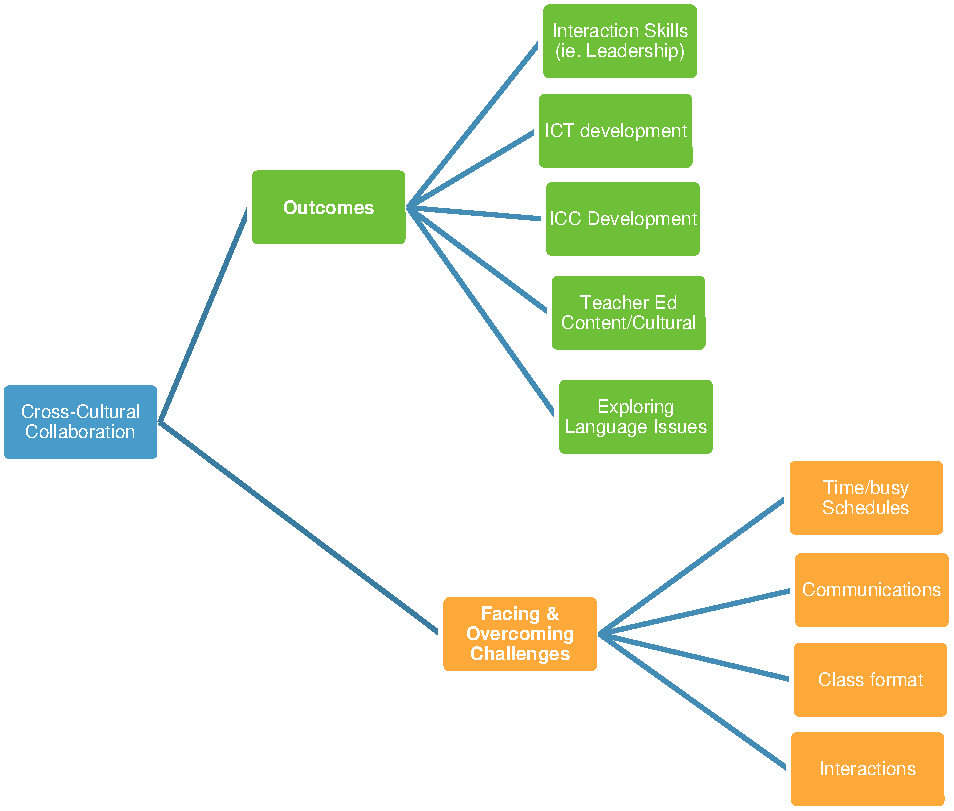
\includegraphics[width=\textwidth]{figure01.pdf}
\caption{Cross-Cultural Collaboration Outcomes - Facing \& Overcoming Challenges.}
\label{fig-01}
\source{Own elaboration.}
\end{minipage}
\end{figure}


\subsection{Outcomes}\label{sub-sec-outcomes}
\subsubsection{Interactional Skills}\label{sub-sub-sec-interactional}

Participating in a VE Project is a way to develop many attitudes and
skills that place the students in the center of their learning process,
as they are the ones who need to take the initiative, leadership and
autonomy for developing the tasks and collaborations. There is a \enquote{truly
learner-centered pedagogy} and it results in \enquote{increased
student-teacher responsibility} \cite{sadler2016twelve}.
		
In the analysis, it was possible to notice that some teams readily took
the initiative and appreciated the skills learned from the process. The
quote below shows how this group of students worked together to develop
the project: even being physically distant to each other, the digital
platforms enabled connection, sharing of ideas and responsibilities on
the tasks.

\begin{quote}
An initial expectation that I had was that we, as a group, would
communicate on a regular basis and have some sort of plan to dive up
responsibilities so that it would be easier for us to work on our
project. These expectations were absolutely met. We were in constant
contact, and did an excellent job or dividing all of the parts of the
presentation up. (US 2023 ST3-42)
\end{quote}

Collaboration was another aspect shared in most of the
PSTs' answers in the survey. They valued the
interaction they had with students from another part of the world; the
group work itself and the way they shared their responsibilities for
developing the project. This is probably because of the own nature of VE
projects that enable a more student-centered approach. In addition, the
professors' balance of guidance and autonomy in conducting the project
contributed to this collaborative environment.

\begin{quote}
One benefit from this was learning to be more self-dependent and
taking the instructions and collaborating with each other to put the
pieces together (US 2022 ST3-8).
	
My initial expectations for participating was that everyone will
add their input in the project and communicate with one another. These
expectations were met way beyond my expectations because everyone was on
Whatsapp chatting with each other and schedule times to communicate with
everyone with the project and everyone added their parts of the project.
(BR 2023 ST3-41)
\end{quote}

Data also indicated that some teams worked well together. Collaboration
was both a positive outcome as well as a challenge they faced and had to
overcome by applying different negotiation strategies. Some PSTs
reported collaboration in different platforms; shared
responsibilities for the project and the creative element when preparing
together the presentations. Their experiences with
telecollaboration were mixed regarding the ways they felt close or
physically distant to their colleagues. Their answers also pointed out
that they thought about their future roles as teachers when negotiating
actions and working collaboratively with other colleagues, for example:

\begin{quote}
There is something that is a benefit and a challenge at the same time, that I think that helps me becoming a better teacher, which is working in group. Me as a teacher need to know how to choose the best words to interact and make people comfortable to participate and give their opinion. I tried to do that when talking with my partners about the project, I tried to tell my opinion without being rude and being supportive. (BR 2023 ST2-58)
			
A benefit I got from this project is I learned the process of working with other educators. In my future career for example, I can use what I learned from this when working with coworkers to plan/research a unit. (US 2023 ST5-47)
\end{quote}

These quotes demonstrate that the VE Project was a context for
experiencing collaboration and developing some soft skills that are
important for their lives. When interacting with colleagues from
different cultural backgrounds, they learn to take leadership,
negotiate, and deal with conflicts.

According to \textcite{odowd2021virtual}, student’s
learning outcomes in different models of VE Projects across the globe
have to do with the way they feel "better prepared to communicate and
collaborate with people from different cultures". Hurdles or challenges
actually enhance participants' ability to find ways to creatively
collaborate and communicate with partners from other countries. Based on
O'Dowd's suggestion, for the two years of this VE project, professors
carefully designed tasks to push students out of their comfort zone, but
professors also carefully monitored the process and stayed in touch
daily to guide some PSTs who needed reminders or other support.
		
\subsubsection{ICT Development}\label{sub-sub-sec-ictdevelopment}

In a previous paper, the authors of this text identified both the
benefits and challenges of ICT during the VE Project. The following
benefits stood out: the critical nature of technology for the
communications; having choices of platforms; the uses of both
synchronous and asynchronous forms of technologies; opportunities to
help each or use trial and error learn new technologies; learning new
technologies that are used in each culture; getting to know other
students from other countries through ICT. On the other hand, the
challenges were related to time, access to the internet or internet
connection; getting in contact (i.e., email and not getting
response /communication) with everyone; and difficulties with specific
platforms. Though the authors emphasized that there were more benefits
than challenges; dealing with the challenges was important for the PSTs
to develop attitudes in their professional lives as well as for the
professors to consider important aspects of ICT when planning their
virtual collaborations \cite{calvo2023investigating}.

\begin{quote}
Having WhatsApp made the project go very smoothly. It was a great
asset to have in order to communicate with others across the world. I
remember discussing this project with my parents, and they told me how
lucky I was that we had phones and technology to do so, because when
they were younger, they had pen pals they would communicate with by
letters! I am very grateful to have had the technology to meet and work
with the girls in my group. (US 2023 ST3-42)

The benefits of technologies were the opportunity to be able to
communicate with people from another country, in addition to the ease of
access to information about who we worked with during the project, in
addition to easy access to learning from different contexts. One of the
difficulties was how to learn to use the voice thread, because, besides
the tutorial we had in the classroom, that platform is complex to use
and we had to do some steps that weren’t in the tutorial
to publish our presentation. (\emph{BR 2023} ST2-59)
\end{quote}

For both students, the technology itself was indispensable for the
interactions to happen. Besides valuing and recognizing its role in
recent educational practices, BR 2023 ST2-59, for example, also
mentions the difficulties with a specific platform, the VoiceThread.
This specific difficulty may have helped the PST to search, learn more
and use this platform.

\subsubsection{Intercultural Communicative Competence (ICC) Development}\label{sub-sub-sec-intercultural}

While seven weeks of collaboration could yield only limited shifts in
such ICC skills as mindfulness, cognitive flexibility, and impacts of
second language acquisition \cite{idris2019intercultural,uzum2020using}, 
PSTs shared some memorable aspects of the cross-cultural
collaborations, such as motivation for the intercultural encounters,
sharing experiences, learning and respecting differences.

The analysis showed that students expressed motivation for interacting
and learning with each other. The exchanges allowed them to have contact
with people with different stories and life experiences. Often a first
step towards ICC is developing self-knowledge, by listening to others to
consider how we are different and similar. Direct and thoughtful
encounters with people, places, and foreign languages such as through VE
with students at other colleges are effective ways to begin to develop
ICC \cite{idris2019intercultural,lopez2017developing}, as PSTs in the
study indicated:

\begin{quote}
I could saw how important is try to have a contact with people
from other countries and cultures, because we can learning a lot sharing
experiences, and we can also learn to be more respectful in face of
differences. (BR 2022 ST1-26)

I think this project really showed us just how valuable it is to
learn from people that are different from us. There were many times when
we just had random group conversations, just discussing our lives, and
providing insight into the differences in our lives. (US 2023 ST3-42)
\end{quote}

\subsubsection{Content Learning and contextual information about the countries}\label{sub-sub-sec-content}
	
Data indicated that PSTs not only pointed out the contents they learned
during the VE, but they mentioned how they could learn them in a
cross-cultural way, comparing and analyzing them according to the
contextual information and reality of the two countries.

\textcite{odowd2021virtual} also found that cultural knowledge was
developed though VE Projects. According to him, in some situations,
students mentioned the factual information they learned about many
social aspects. In addition, students pointed out the development of
cultural awareness about diversity in a way to "avoid regarding cultures
as monolithic". Similarly, \textcite{kopish2020leveraging} found that students
in their study were learning from cultural experiences very different
from their own and what helped them was their desire and ability to
identify with new cultural partners.

\begin{quote}
One of the benefits of the project for my teacher education
process was to learn about the teacher education from different context
and the difference and similarities between both contexts. This is
really important for our formation, because there is not only one way
that is correct, it really depends of the culture and aspects that we
are inserted. (BR 2023 ST2-59)

The benefits would be that it allowed us to view English education
and ELLs from a different perspective, as these pre-service teachers are
all specifically going to be English teachers but a lot of the students
at [university] are going to be educators in a different subject,
but are still required to take courses that are necessary for teaching
ELLs. (US 2022 ST4-1)
\end{quote}
	
\subsubsection{Exploring Language Issues}\label{sub-sub-sec-exploring}

For many Brazilian PSTs, their English language skills were developed
and when interacting with PSTs from another context, they had
opportunities to experience language use situations that are different
from classroom activities. As all the Brazilian students were from the
Letras program (Language Arts undergraduate program), most of them were
fluent in their English communication as the VE tasks and interactions
were developed in this language.

The following illustrates the way this Brazilian PST was initially
worried about correctness; then mentions some other aspects that are
more relevant in communication (e.g. getting the message across;
negotiating meaning) that would be more important to consider in this
kind of interaction.

\begin{quote}
I could learn many things with my group. The communication was of
course a challenge for me, because I was afraid and worried about
texting correctly. Some days after, I stopped to worry about the grammar
of my written messages on WhatsApp. If my partners did not understand
something, I’ll text and write again. (BR 2023
ST4-66)
\end{quote}

Also, when participating in VE initiatives, participants may also
evaluate in different ways their linguistic competence, as one Brazilian
PST shared: \enquote{These projects clearly help the students to be proud and confident in their speeches}. (\emph{BR 2023 ST2-56}). In this
regard, \textcite[p. 217]{odowd2021virtual} found that different from
traditional ways of learning languages that are focused more on
accuracy, in telecollaborative opportunities students use the language
in a meaningful way.

PSTs from the US university related to other aspects of languages. For
example, they mentioned the role of languages in society such as: how
languages affect schools and other contexts, how other speakers are
fluent in English, how only fluency in English is not enough to avoid
misunderstandings, and their future work as teachers of bilingual
students.

\begin{quote}
[$\ldots$] The number of students from other countries both in my
school and in Brazil that were fluent in English surprised me. The
project just reinforced why it’s so important to be
bilingual and use one language to learn another. The other students were
using what they knew to understand our differences. The experience
exceeded that expectation. (US 2023 ST2-36)
	
It also highlighted how it can sometimes a language barrier can
pose a problem, even if both parties are fluent or almost fluent in a
language. There was a point where we set up a meeting, but because of
confusion based on our language differences, we met at different times
and missed our meeting. I think this could be translated to teaching
emerging bilingual students. It just opened my eyes to how beneficial
working with people who speak other languages can be, but also the
difficulties that remain. (US 2023 ST3-42)
\end{quote}

Participating in VE Projects are important initiatives not only to
develop language skills, but to understand and consider language use and
learning in a different perspective. In those excerpts, ST2-36
highlights the important way he sees the bilingual speaker using the two
languages to understand and make meaning of the experience. In the
second excerpt, ST3-42 calls the attention to the fact that fluency in
the language is only one aspect in communication - even being fluent in
their communication to schedule a meeting, they missed it because none
of the US or BR students paid attention to the time zone differences in
the countries. So, by this example, we can notice that communication is
more than just using words; it also has to do with negotiating meaning.

\subsection{Facing Challenges} \label{sub-sec-facing}
\subsubsection{Communication, interaction and collaboration}\label{sub-sub-sec-communication}

PSTs most often mentioned challenges were related to communication,
interaction, and collaboration. Some teams did not feel the
participation or initiative by some members met their expectations,
mostly due to the US PSTs in those teams not responding right away to
the Brazilian students' attempts to communicate and work on the
projects. This was probably due to the fact that the US students were
not used to communicating with WhatsApp as the Brazilian students were;
so, this cultural difference in terms of technological tools for
interaction had an impact in the initial phase of the project.

This difficulty in communication affected their organization to start
working on their projects. The Brazilian PSTs complained about the
\enquote{initial silence} from the US PSTs. Data indicated, though that soon
after getting in touch with each other, some groups could work well
together and share the responsibilities. While they were delayed with
initial responses to Brazilian PST's emails, ironically, several US PSTs
expressed that they wanted to have some more time for interactions, so
email was not the best way to start this cross cultural collaboration.
	
\begin{quote}
[$\ldots$] we did not have as much communication as I would have
liked or have expected. I do think it was interesting to talk to the
students and enjoyed what little conversations we did have. (US 2022
ST3-8)
		
I would say that one challenge that I had was communication. I had
some difficulties communicating with the rest of the group and I believe
that this could've been mitigated if there was more in person
communication. At least for me personally considering I am not the
greatest at seeing my emails. (US 2023 ST5-50)
\end{quote}
	
\subsubsection{Time and busy agendas}

Most PSTs found ICT solutions to work through the challenges of busy
schedules, time zone differences (2 hours difference) and communication
with everyone. They learned to adapt and use WhatsApp for group
communication, as an asynchronous platform for group activities/tasks
even if this was their first time learning the App.
	
\begin{quote}
[\ldots] getting ahold of everyone was difficult. For example,
our group member emailed us on to create a WhatsApp, and one of our
group mates didn't respond until [2wks later]\ldots. communication
was difficult, even with some of the students at [Univ.] because we
were all on different campuses with different schedules\ldots.but we
used resources like WhatsApp and google slides to help us communicate
with one another. I had never used WhatsApp before this assignment, so
learning how to use that app was beneficial in case I ever need to use
it again. At first, it was difficult to get a steady communication
source with everyone. However, we got it all figured out by the time our
presentation was due. (US 2022 ST3-2)
\end{quote}
	
Providing both required ICT and developing a well-planned and guided VE
framework \cite{gleason2021design} as well as allowing
students to choose their ICT, supported the development of ICC \cite{kolm2022international}. PST in this study showed they were developing
skills for communication through asynchronous and synchronous
technology, leadership, project management, and cultural diversity
through different forms of technology. Besides their busy agendas, the
class format of the classes in the two contexts had and impact on the
development of the activities. The next section explores this challenge
in the VE project.

\subsubsection{Class format}\label{sub-sub-sec-class}

Another factor that impacted the cross-cultural collaboration was the
class format; while Brazilian students had in-person classes, US
students had asynchronous web classes. So, the ways that professors
interacted with PSTs were also different; the US professor needed to
follow the development of the tasks and interactions by continuous
online check-in with their students, while the Brazilian professor had
classes with their students twice a week and gave those PSTs some class
meetings to develop activities for their respective cross-cultural
projects. Considering these differences, though, PSTs felt supported.
This Brazilian PST recognized the collaboration process among the
professors to organize the VE.

\begin{quote}
Professor [Brazil] has been very supportive and understandable
since we started this program, and so they always made it very clear
that they constantly wanted to check our work in progress, by giving
ideas, embracing others we had, and that they was always in contact with
Professor [US], who was nothing but receptive and empathetic. I
really appreciate the fact that \textbf{they} are really interested in
our culture, knowing so much about it, and being open to our suggestions
too. (BR 2023 ST4-65).
\end{quote}

This collaboration was also seen in the study of \textcite[p. 412]{sadler2016twelve} with their PSTs. The authors emphasize the mutual
responsibilities and VE joint planning/ development by the teachers. In
this way their students could see their collaboration and the use of
telecollaboration in their practices.

Because of this class format difference, the US professor took into
consideration the importance of additional asynchronous virtual
scaffolding and explanation about the project. Balancing the amount of
scaffolding (reminders about upcoming tasks or reminders to read their
messages from the BR PSTs, extra directions, or video/picture
directions) with supporting and encouraging students’
autonomy was at the forefront of the professors’
consideration when planning and implementing the VE tasks.





\section{Conclusions}\label{sec-conclusions}

One of the main types of evidence of this study has been the
confirmation of the great difference that exists between the number of
news published in all media about traffic accidents (89.14\%) compared
to the other three causes studied.

In addition to this important data, the great finding of this study has
been the confirmation of the high number of accurate headlines that also
fully coincide with the development of the news (27.15\%).

This result suggests that the media are using automated journalism,
directly uploading the information they receive from emergency services
or information agencies, without modifying, working on or adapting the
news at all.

This news production mechanism is used by all the media, to a greater or
lesser extent, with \url{lavanguardia.com} being the media that uses it
the most (66.23\% of all its news on traffic accidents are identical to
those of other media). In total, 663 duplicated, 17 tripled and 6
quadrupled news items have been detected, which means that the same
headline and body of the news item is repeated on up to six occasions in
exactly four media outlets at the same time.

In any case, an analysis has also been carried out on the exact news
published by all these media about other types of events, obtaining
similar results for drowning and accidental falls but observing a
different informative treatment in the case of suicides, where only
11.00\% of coincidences with other journalistic pieces (12 news).

Regarding the results of the qualitative analysis, a dependency of the
media on the notes issued by the emergency services is observed in the
in-depth interviews, although it is stated that a contrast of this
information is carried out before incorporating it as a publication.

It is indicated that the news of events are published to a greater
extent because they arouse interest in the audience and that the
sensitive data of the victims is taken into account in their production.

On the other hand, the discussion group believes that journalistic work
is carried out superficially and, in the case of suicides, without
social commitment. Regarding this first statement, the fact that more
and more traffic news is being published automatically seems to prove
them right.

Therefore, taking the agenda-setting theory as a basis for reflection,
where the media influence the issues that concern and speak of citizens
-in this case, events-, it seems that they have finally managed to shape
the public agenda so that the citizens talk preferentially about traffic
accidents over other types of events \cite{scheufele2007framing}.

In view of all these special characteristics described, it can also be
seen that there is automated journalism in the writing of traffic
accident news, which in most cases are automatically reported from the
emergency services to the media themselves without adapt the news
neither to its editorial line nor to its audience.

In short, attention must be drawn to the vicious circle that can be
generated if the media continue to offer exhaustive information on
traffic accidents, while ignoring the reality of some events that also
represent a social problem.

\printbibliography 

\begin{contributors}[sec-contributors]
\authorcontribution{Luciana Cabrini Simões Calvo}[conceptualization,datacuration,formalanalysis,investigation,projadm,validation,visualization,writing,review]
\authorcontribution{Lynn C. Hartle}[conceptualization,datacuration,methodology,projadm,validation,visualization,writing,review]
\end{contributors}

\end{document}
